\documentclass[10pt,xcolor=pdflatex,hyperref={unicode}]{beamer}
\usepackage{newcent}
\usepackage[utf8]{inputenc}
%\usepackage[czech]{babel}
%\usepackage[T1]{fontenc}
\usepackage{hyperref}
\usepackage{fancyvrb}
\usetheme{FIT}

%%%%%%%%%%%%%%%%%%%%%%%%%%%%%%%%%%%%%%%%%%%%%%%%%%%%%%%%%%%%%%%%%%
\title[WEBOVÝ EDITOR PREZENTACÍ]{WEBOVÝ EDITOR PREZENTACÍ}

\author[]{Adam Abrahám}

\institute[]{Fakulta informačních technologií
Vysokého učení technického v Brně\\
Bo\v{z}et\v{e}chova 1/2. 612 66 Brno - Kr\'alovo Pole\\
xabrah04@vutbr.cz}

\date{} % bez data / without date

%%%%%%%%%%%%%%%%%%%%%%%%%%%%%%%%%%%%%%%%%%%%%%%%%%%%%%%%%%%%%%%%%%

\begin{document}

\frame[plain]{\titlepage}

\begin{frame}\frametitle{Existujúce riešenia}
    \begin{itemize}
        \item \emph{Marp}
        \item \emph{Swipe}
        \item \emph{HackMD}
    \end{itemize}
    
    \vspace{\baselineskip}
    \vspace{\baselineskip}
    \emph{Výhody}: Zadarmo, Online, Verzovanie, Kopírovanie snímok
\end{frame}

\begin{frame}\frametitle{Použité technológie}
    Databáza:
    \begin{itemize}
        \item \emph{MongoDB}
    \end{itemize}
    \vspace{\baselineskip}
    
    Frontend:
    \begin{itemize}
        \item \emph{Vue.js/Nuxt.js}
        \item \emph{Reveal.js}
    \end{itemize}
    \vspace{\baselineskip}
    
    Backend:
    \begin{itemize}
        \item \emph{Node.js/Express.js}
    \end{itemize}
    \vspace{\baselineskip}
    
    \begin{itemize}
        \item \emph{REST API}
        \item \emph{TypeScript}
    \end{itemize}
\end{frame}

\begin{frame}\frametitle{Architektúra aplikácie}
    \begin{figure}[!hbt]
        \centering
        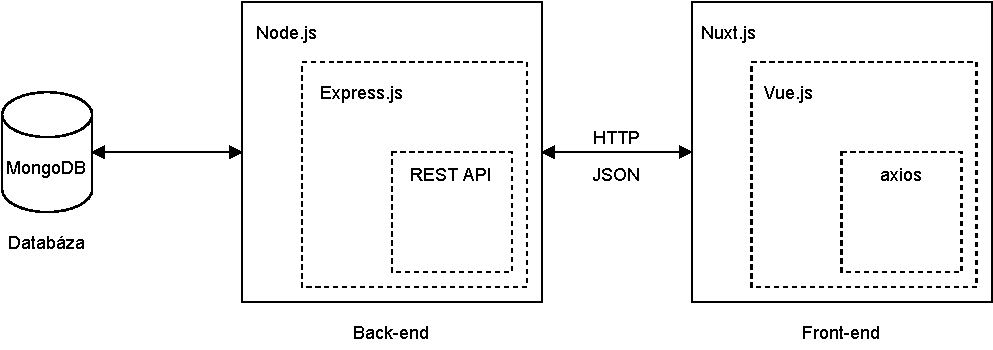
\includegraphics[scale=0.60]{img/architektura.pdf}
    \end{figure}
\end{frame}

\begin{frame}\frametitle{Implementácia}
    \emph{Nuxt.js}
    \begin{itemize}
        \item Autentifikačný modul
        \item Smerovanie
    \end{itemize}
    \vspace{\baselineskip}
    
    \emph{Perzistentné úložisko}\\
    \vspace{\baselineskip}
    \emph{JSON Web Token}
\end{frame}

\begin{frame}\frametitle{Testovanie aplikácie}
    \emph{Postman}
    \vspace{\baselineskip}

    \emph{Cypress(E2E)}
    \begin{figure}[!hbt]
        \centering
        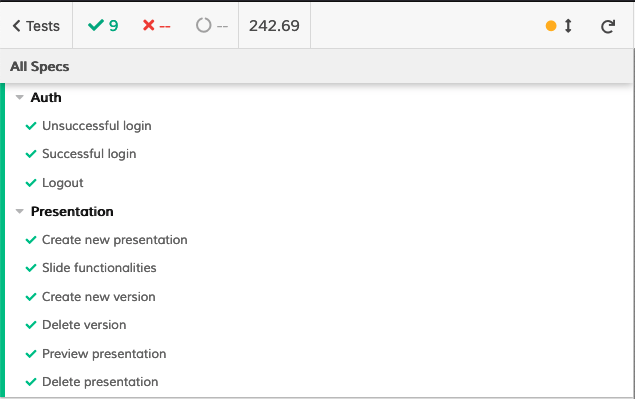
\includegraphics[scale=0.3]{img/cypress.png}
    \end{figure}
\end{frame}

\begin{frame}\frametitle{Domovská stránka}
    \begin{figure}[!hbt]
        \centering
        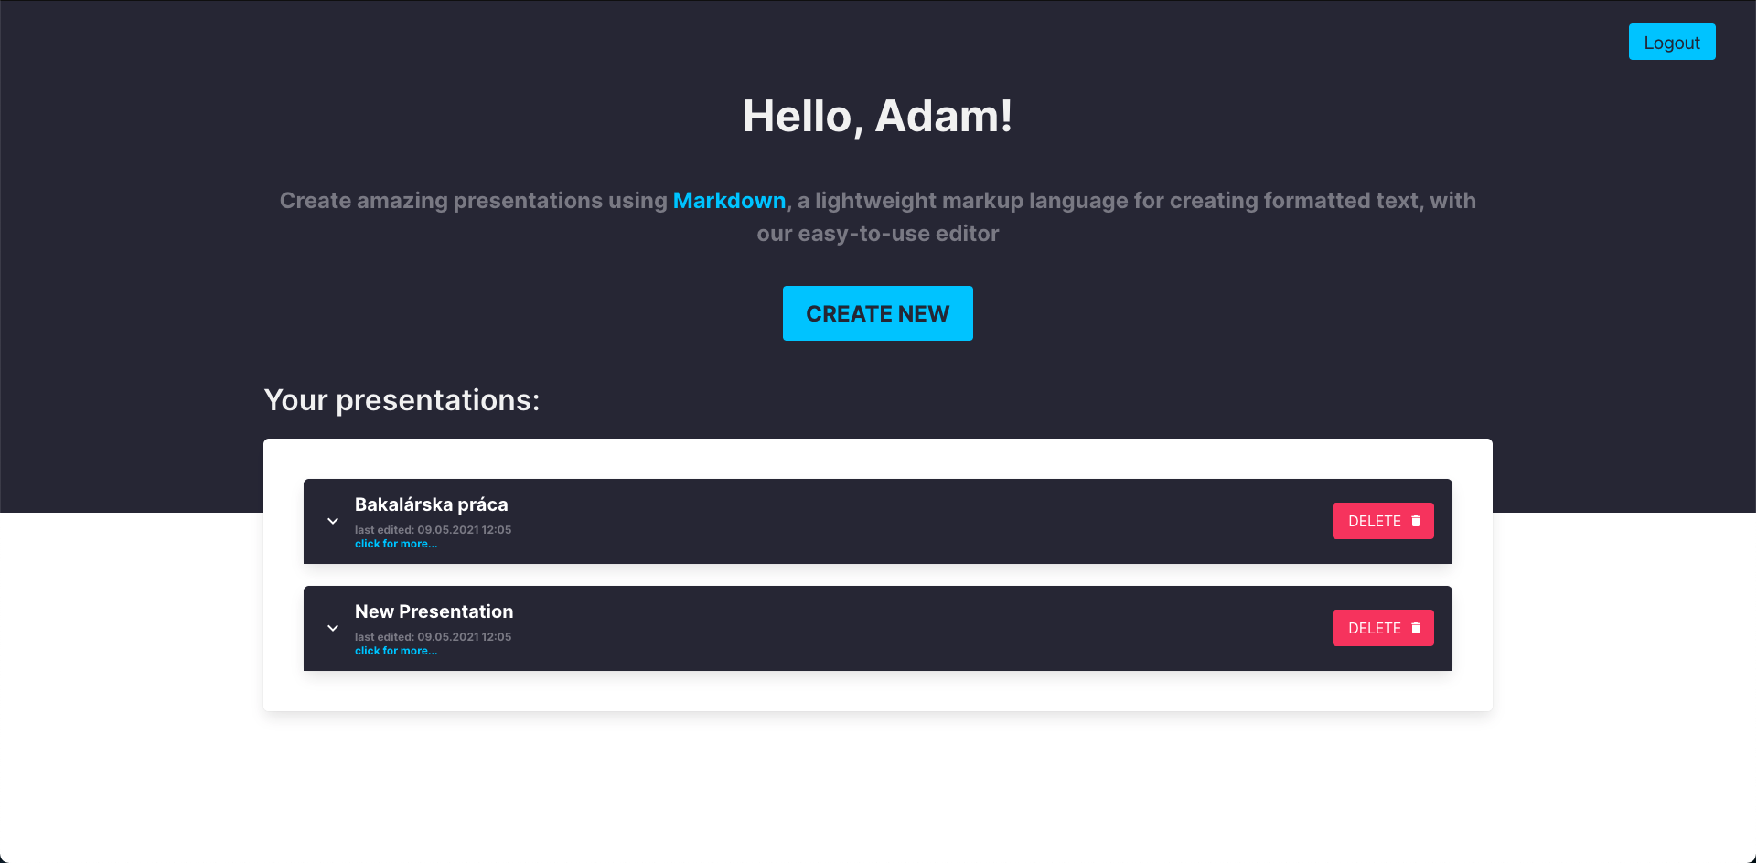
\includegraphics[scale=0.35]{img/domovska_stranka.pdf}
    \end{figure}
\end{frame}

\begin{frame}\frametitle{Detail prezentácie}
    \begin{figure}[!hbt]
        \centering
        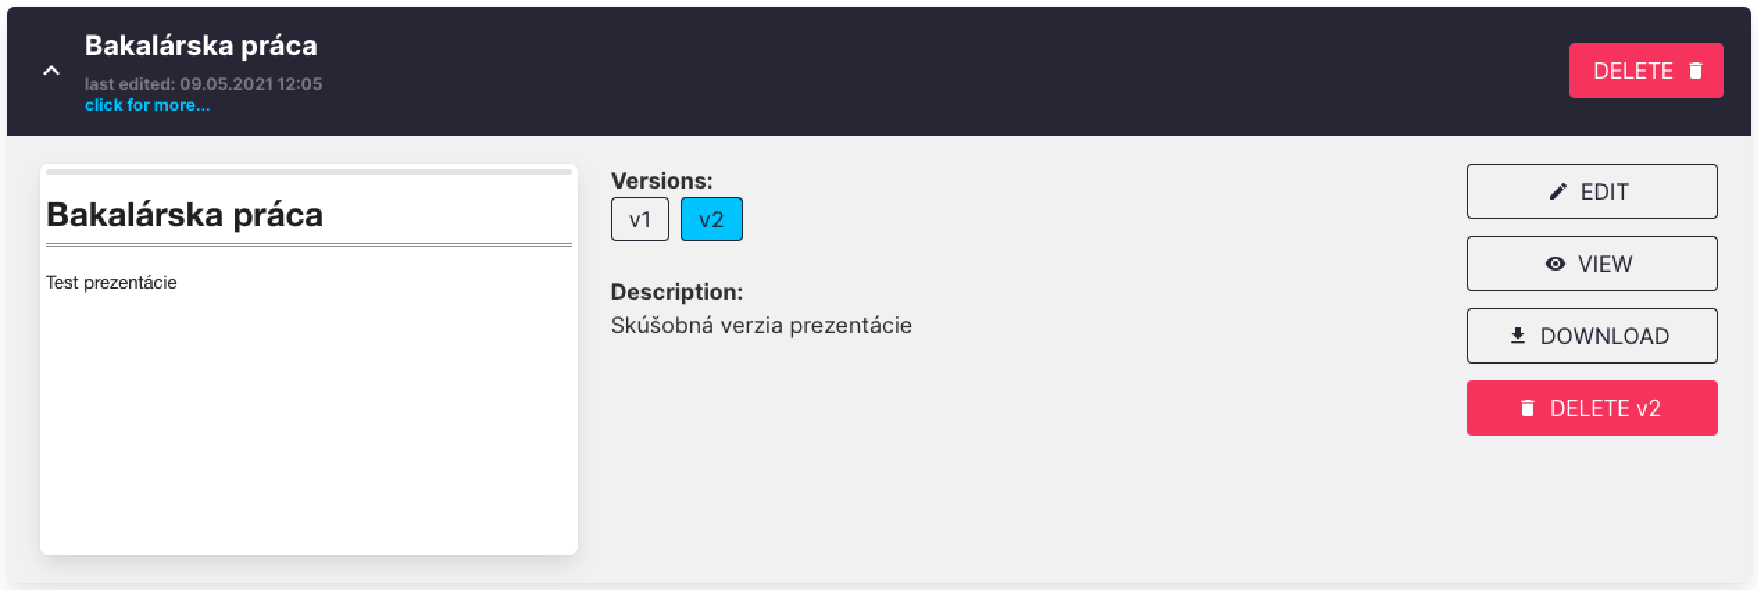
\includegraphics[scale=0.35]{img/detail_prezentacie.pdf}
    \end{figure}
\end{frame}

\begin{frame}\frametitle{Editor}
    \begin{figure}[!hbt]
        \centering
        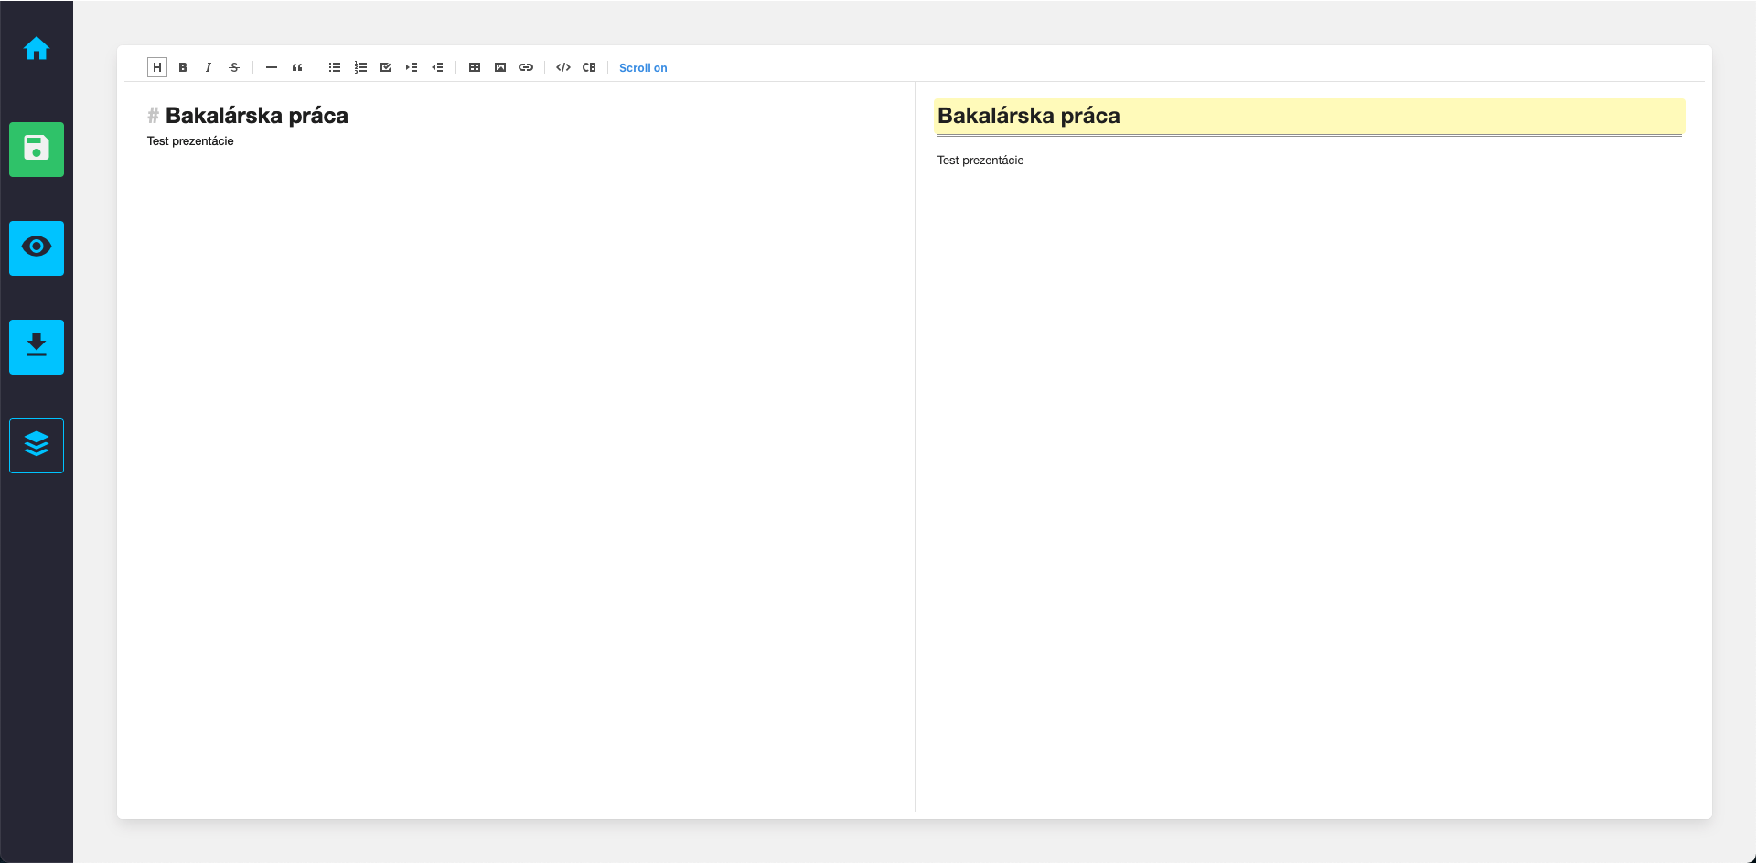
\includegraphics[scale=0.35]{img/editor.pdf}
    \end{figure}
\end{frame}

\begin{frame}\frametitle{Bočný panel}
    \begin{figure}[!hbt]
        \centering
        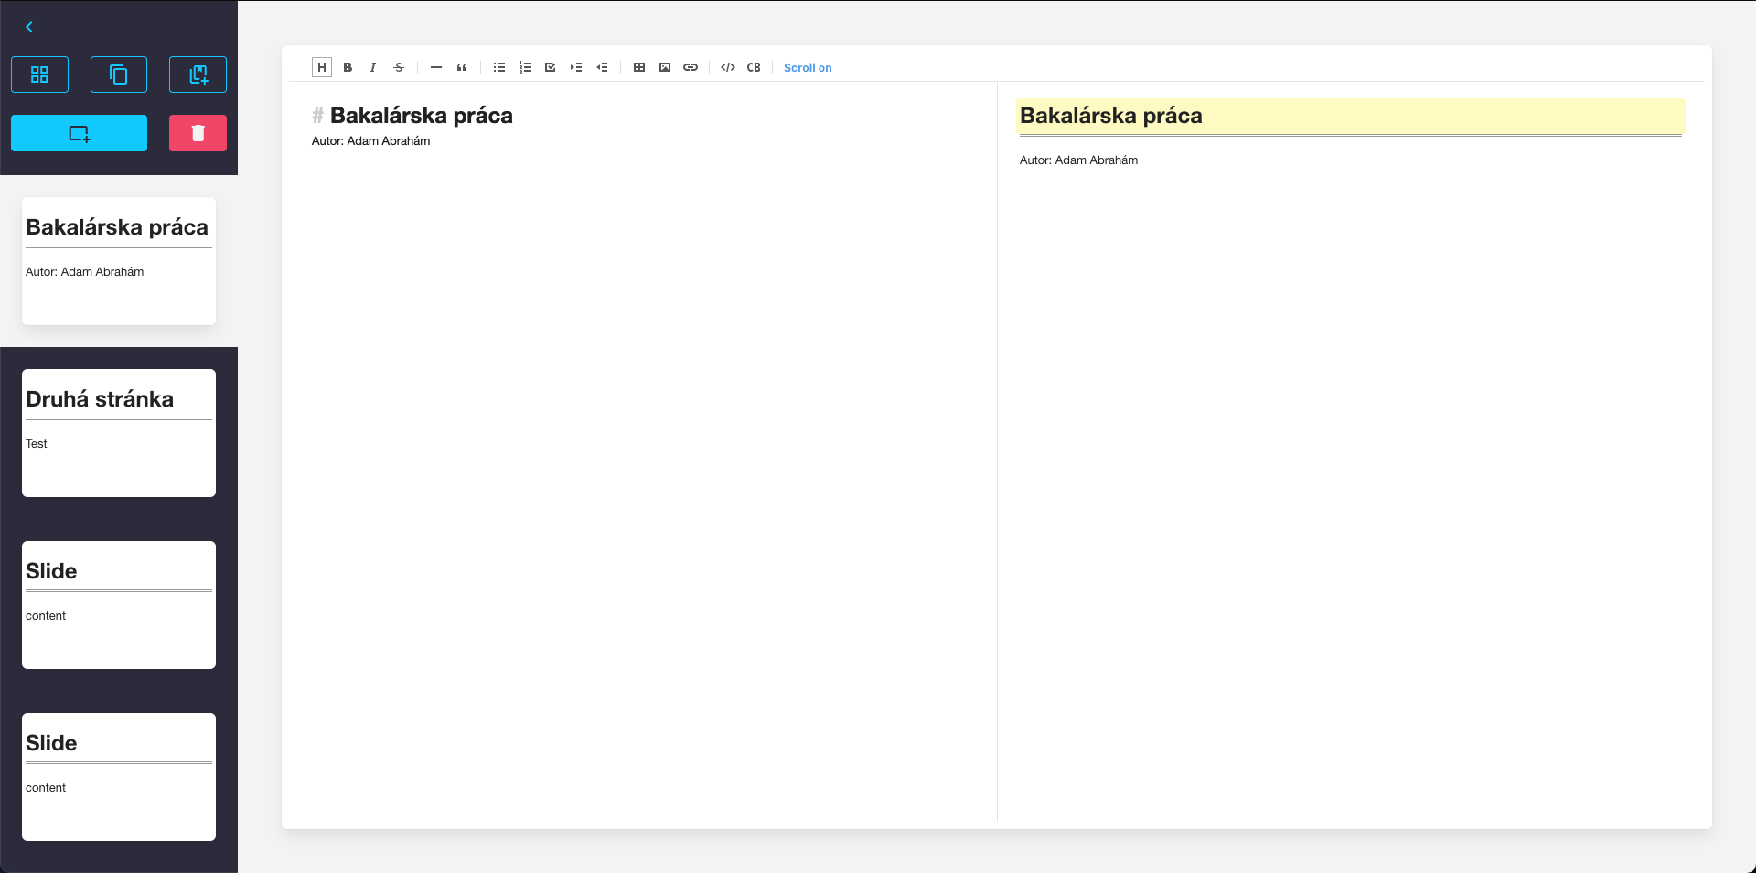
\includegraphics[scale=0.35]{img/bocny_panel.pdf}
    \end{figure}
\end{frame}

\bluepage{Ďakujem Za Pozornosť!}

\begin{frame}\frametitle{Otázka od oponenta}
    \emph{    Bylo by možné vámi vytvořený systém rozšířit o některé další funkce, jako např. vizuální styly jednotlivých snímek nebo animace? Pokud ano, jak složité by to bylo a jak by to bylo možné realizovat?}
    
    \begin{figure}[!hbt]
        \centering
        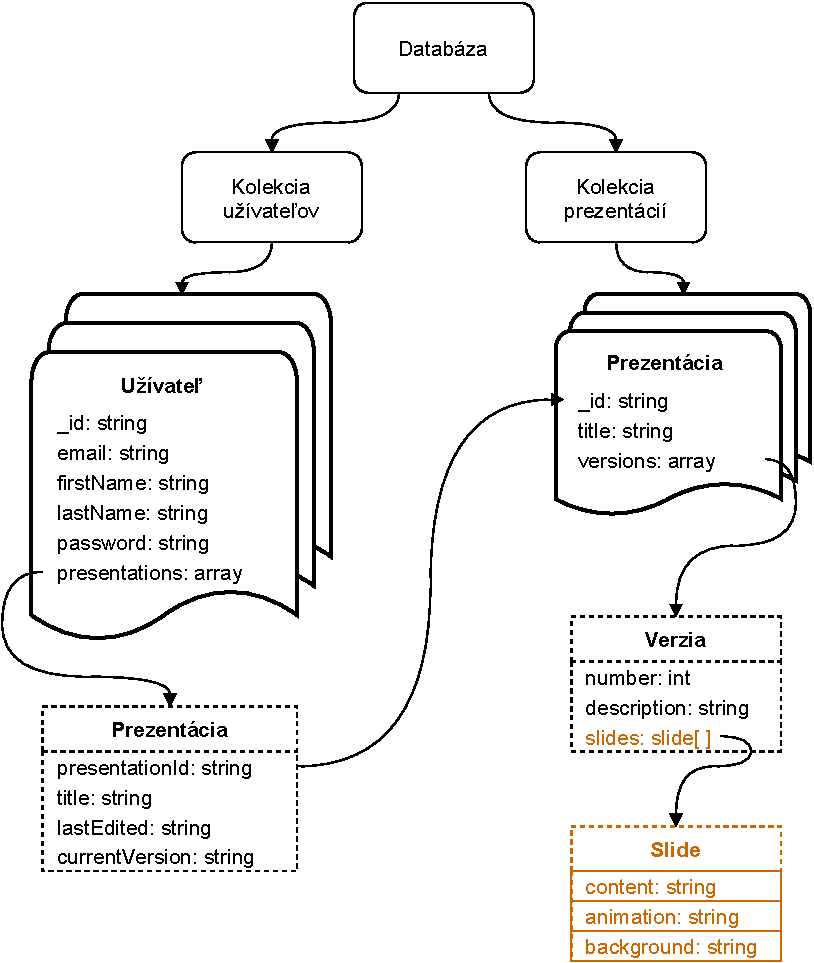
\includegraphics[scale=0.4]{img/databaza-1.pdf}
    \end{figure}
\end{frame}

\end{document}
